\documentclass[12pt]{article}

\usepackage{geometry}
\geometry{a4paper}
\geometry{margin=2.5cm,top=2cm,bottom=2cm}

\usepackage{lastpage}
\usepackage{fancyhdr}
\pagestyle{fancy}
\renewcommand{\headrulewidth}{0.4pt}
\renewcommand{\footrulewidth}{0.4pt}
\renewcommand{\sectionmark}[1]{ \markright{#1}{} }
\lhead{Cyril NOVEL (cbn13)}\chead{}\rhead{\textit{ \nouppercase{\rightmark}}}
\lfoot{}\cfoot{\thepage\ of \pageref{LastPage}}\rfoot{}

\setlength{\headheight}{15pt}

\usepackage[english]{babel}
\usepackage[utf8]{inputenc}
\usepackage{amsmath}
\usepackage{graphicx}
\usepackage{algpseudocode}
\usepackage{algorithm}
\usepackage{amsthm}
\usepackage{amssymb}
\usepackage{mathtools}
\usepackage{commath}
\usepackage{stmaryrd}

\title{OFusion\\
\large{CO542 Individual Project}}

\author{Cyril NOVEL}

\date{\today}

\begin{document}
\maketitle
\newpage

\tableofcontents

\newpage

\addcontentsline{toc}{section}{Introduction}
\section*{Introduction}
Augmented reality is a dynamic field in Computer Science and Computer Vision, with the multiplication of portable devices with high perfomance CPU and GPU. Multiples devices are providing an augmented reality experience. The Nintendo 3DS has a dedicated game with augmented reality cards, applications can be downloaded on smartphones. The Google Glass works like a small Head Up Display for the user, similar to what can be seen in some videogames. The Project Tango phone and tablet comes with built-in augmented reality applications. However, none of these devices are capable of displaying information for the entire field of view of the user. The smartphone or tablet size is small compared to the size of the field of view. The Google Glass encounters the same problem: there is no possible overlay of the reality.

By using a virtual reality headset, such as the Oculus Rift, we cover the entire field of view of the user. Using an appropriate sensor, we can understand the scene surrounding the user. Then we can overlay information on the reality for the whole field of view. This creates a new kind of augmented reality device. Applications are infinite: the road to follow can be directly highlighted in a GPS application; you can play a virtual game in your living room with the game understanding the geometry of your living room -- making each game unique since you can move objects; a medical application can highlight organs during an operation and also provide an HUD with useful information. Possibilities are countless.

During this project, we created a device fusionning an Oculus Rift and a Kinect to create a new kind of augmented reality device. The Kinect captures the surrounding scene. It is then rendered in 3D in the Oculus Rift with real-time color information. Thus the user can evolve just like in real life. An augmented reality application has been integrated. Using a \textit{magic pen}, it is possible to draw virtually on a surface.
\newpage

\section{Hardware review}
\subsection{Virtual reality headsets}
A virtual reality headsets is a device capable of displaying 3D scenes to the user wearing the headset. It is made of screen and two lenses, with the left part of the screen showing the image for the left eye and the right eye for the right part.

Virtual reality headsets have been fancied a long-time and are finally becoming reality. The Oculus Rift is the first affordable headset to encounter a commercial success. Previously, Nintendo tried to sell a virtual reality headset called the Virtual Boy. It was a failure since its use caused terrible headaches to the players and only 5 shades of red were available.

In the following sections, we will present some virtual reality headsets and highlight their differences.

\subsubsection{Oculus Rift and Sony Morpheus}
The Oculus Rift is developped by Oculus VR. It is the first virtual headset targetting the mass market, and therefore has an aggressive price -- the first development kit costs 300\$, 350\$ for the second one.

The Oculus uses a screen for displaying the image. In the first development kit, the resolution of the screen was 1280x800, leading to an effective 640x800 per eye. One part of the screen displays the image for one eye, the other part displays the image for the other eye. The Rift uses lenses to distort the image on the screen, so that it fits the actual field of view of the human eye. The field of view of the Rift is 90 degrees horizontally. Figure~\ref{oculusback} shows the back of the Oculus Rift.

Gyros, accelerometers and magnetometers are combined in the helmet in order to track the user's head movements. The first development kit is however unable to detect translation movement.

\begin{figure}[h]
  \centering
  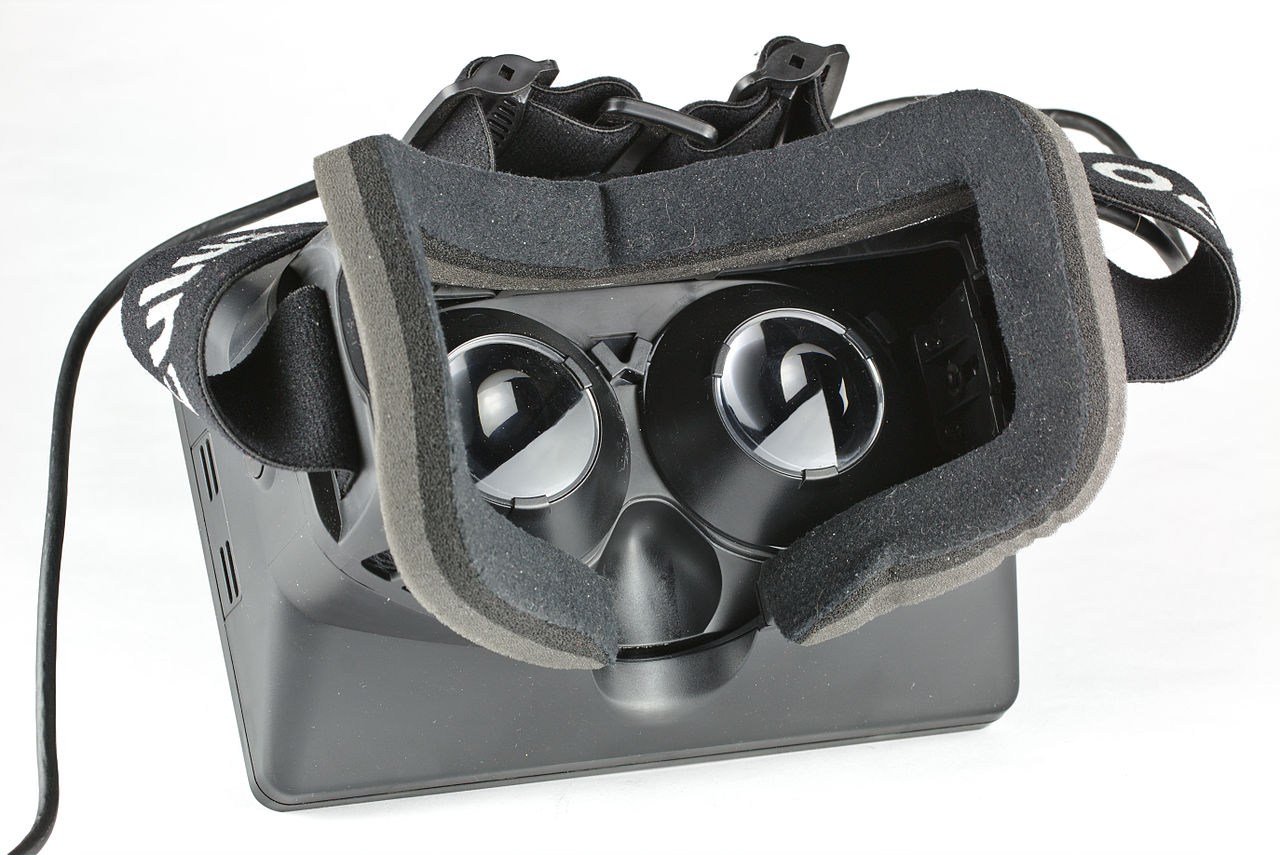
\includegraphics[scale=0.2]{OculusBack.jpg}
  \caption{\label{oculusback} The Oculus Rift}
\end{figure}

The major drawback of the Rift is the resolution of the screen. The screen-door effect is predominant and prevent a total immersion in the displayed scene. The second version of the Development Kit comes with a resolution of 960x1080 per eye, decreasing this effect. This next version comes also with a camera, tracking the movement of the head, in order to detect translation in addition to rotation.

The success of the Oculus Rift leads other companies to develop similar devices. Sony presented few months ago the project Morpheus -- shown in figure~\ref{morpheus}, highly similar to the Oculus Rift.

\begin{figure}[h]
  \centering
  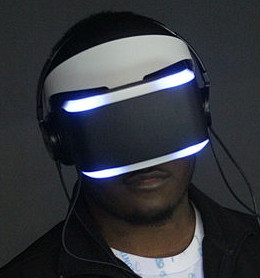
\includegraphics[scale=0.3]{Morpheus.jpg}
  \caption{\label{morpheus} Sony Morpheus}
\end{figure}

Sony Morpheus uses a comparable technology to Oculus Rift. The most noticable difference is that Morpheus has tracking technology all around it, whereas Oculus Rift only has tracking captors on the front and on the sides of the display.

\subsubsection{Google Cardboard and Samsung Gear VR}
During the Google I/O 2014, Google introduced the Cardboard Project. The idea is to use a smartphone as the screen for the headset and create the headset from a cardboard. Google presented the project as a Do-It-Yourself headset, acknowledging that the most difficult part was purchasing the lenses. The design files are available online and some online stores sell and ship the set for 25\$.

\begin{figure}[h]
  \centering
  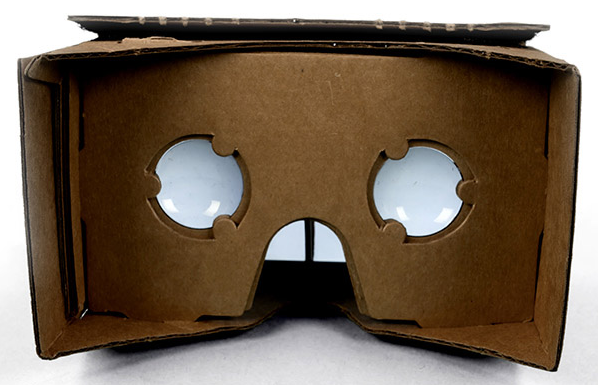
\includegraphics[scale=0.3]{GoogleCardboard.png}
  \caption{\label{cardboard} The Google Cardboard project}
\end{figure}

The advantage of Google Carboard is that it uses the sensors in the smartphone for the head positionning. Every recent smartphone is equiped with a gyroscope and a magnetometer, so the head tracking is easy to achieve.

Samsung is developping a similar headset called Gear VR. Little information are available at the moment but the Gear VR is based on the same idea as Google Cardboard.

The main advantage of smartphones is the high pixel density of the screen. The LG G3 offers a 538 ppi screen, when the first Oculus Rift development kit has \textit{only} a 216 ppi screen. This high density screen counters the screen door effect.

\subsubsection{Vrvana Totem}
The Totem, developed by Vrvana, is similar to the Oculus Rift, except that two cameras are embedded on the front of the headset -- see figure~\ref{tpg}. The idea is that each camera captures the view of one eye.

\begin{figure}[h]
  \centering
  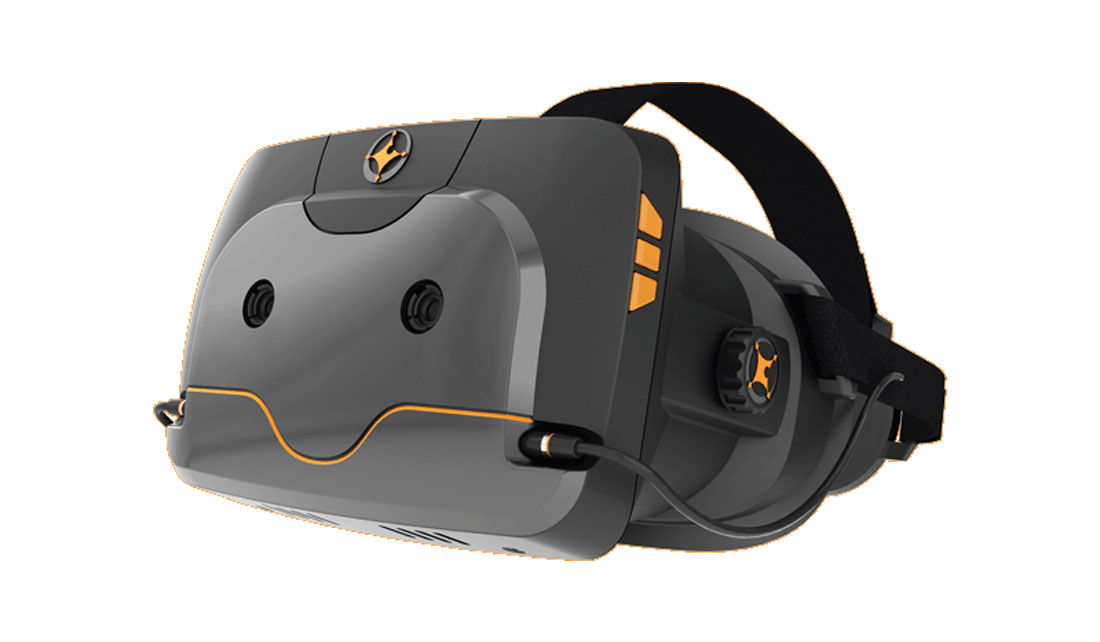
\includegraphics[scale=0.3]{TruePlayerGear.jpg}
  \caption{\label{tpg} The Totem, with two cameras}
\end{figure}

The lens distorsion is computed directly via the hardware in the headset. The others characteristics are higly similar to the Oculus Rift. The Totem is very interesting thanks to these embedded cameras. We want to achieve a new type of augmented reality. The Totem directly captures what the eyes would see. This guarantees an almost perfect 3D image for the user. However, the 3D reconstruction is more difficult - as seen in section~\ref{subsec:stereocam}.

\subsection{Capturing the scene}
For rendering the scene in a virtual reality headset, we need to capture the scene surrounding the user. We can not just extract features from the scene. We need dense information about the scene in real time in order to create the corresponding 3D surface. In this part we present different devices that can compute a point cloud in real time.

\subsubsection{Structured light scanning}
Structured light scanning is a technique used for computing a depth map from the projection of near IR light patterns on the scene. The device project an IR light pattern on the surface of the room. Depending on the depth of the objects, the pattern is bigger or smaller than the reference pattern. Thus we can infer a depth map by reading the projection of the IR pattern. An exemple of pattern is presented in figure~\ref{kinectir}.

\begin{figure}[h]
  \centering
  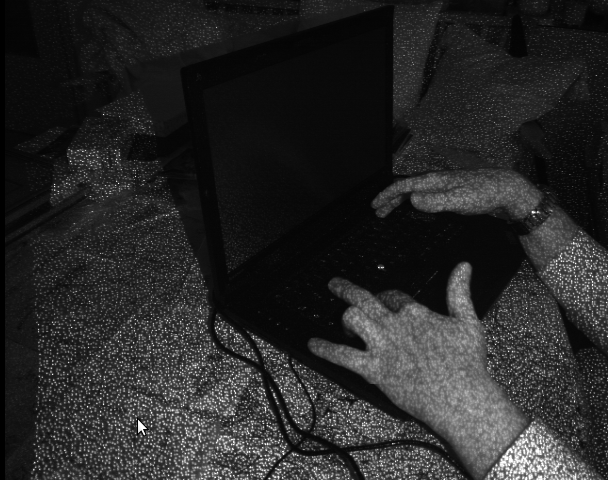
\includegraphics[scale=0.3]{Kinect-ir-image.png}
  \caption{\label{kinectir} Kinect IR pattern}
\end{figure}

This technique is used by the first Kinect -- figure~\ref{kinect}. The resolution of the depth map is $320*240$ points. Other devices using this technique exist, such as the Asus Xtion or the PrimeSense Capri sensor.

\begin{figure}[h]
  \centering
  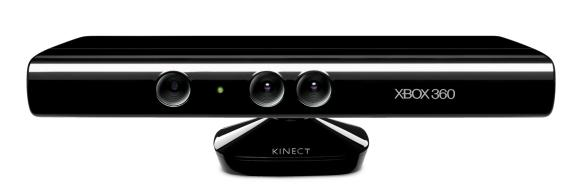
\includegraphics[scale=0.3]{kinect1.jpg}
  \caption{\label{kinect} First Kinect. From left to right: IR Pattern projector, IR Camera for reading the projected pattern, RGB camera}
\end{figure}

It is now possible to create very small IR light projector and IR light captor. The Capri sensor is ten times smaller than the Kinect sensor and can be easily mounted on a tablet or a virtual reality headset. Google Project Tango, a tablet with 3D sensing capabilities, is supposed to use the PrimeSense Capri sensor for capturing 3D information.

However, the use of structured light comes with drawbacks. In very luminous area, the IR light captor can't work because the incoming light is blinding it. Surfaces like TV or computer screen reflect the IR light and so no information can be retrieve from these areas. Finally, the distance between the projector and the captor creates a shadow effect around the object. Very close objects can't be processed since they aren't properly seen by the captor or the sensor. And since the light intensity decreases with the distance, remote objects can't be seen. The computed distance is sometimes wrong for large distances (more than 2 meters). The depth distribution is discrete and coarse for large distance. Beyond two meters, the depth estimation is often considered as unreliable.

\subsubsection{Time of Flight}
A Time of Flight camera is estimating the distance of a point based on the known speed of light. The camera relies on light pulse. The illumination is switched on for a very short time on one point. The light reflects on the object and is gathered by the camera. The delay between the start of the pulse and the gathering by the camera is the time taken by the light to travel twice the distance between the camera and the object. Knowing the speed of light, we can deduce the distance of the point.

Kinect 2 is using a time of flight camera -- figure~\ref{kinect2}. The resolution is much higher than Kinect one, since Kinect 2 produces a $512*424$ depth map. The time of flight doesn't suffer from illumination problems, position problems or distance problems. The depth distribution is not coarse in the remote areas, allowing a nice accuracy of the measurements -- see figure~\ref{depthK2}.

\begin{figure}[h]
  \centering
  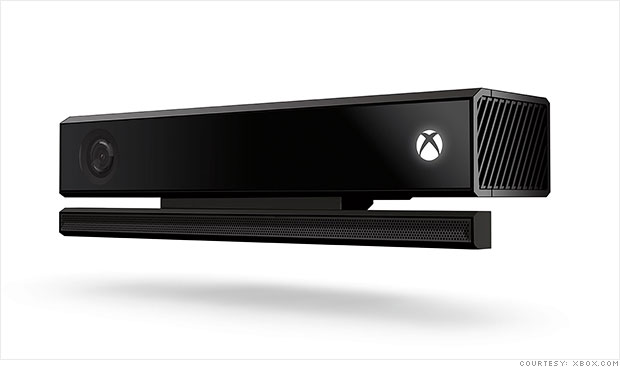
\includegraphics[scale=0.3]{kinect2.jpg}
  \caption{\label{kinect2} Kinect 2}
\end{figure}

\begin{figure}[h]
  \centering
  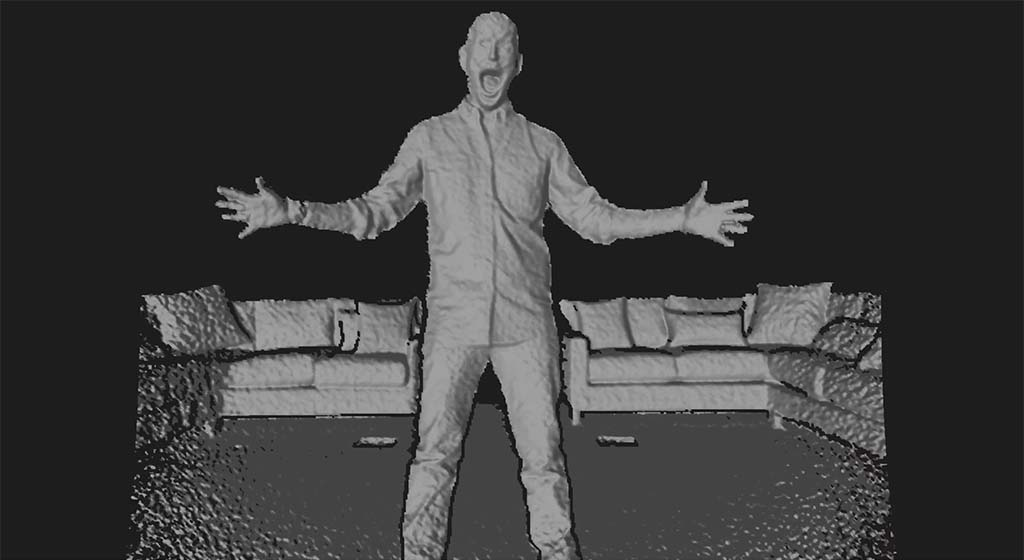
\includegraphics[scale=0.3]{kinect2depth.jpg}
  \caption{\label{depthK2} Depth map with the time of flight camera of the Kinect 2}
\end{figure}

However, Time Of Flight cameras are very expensive, especially for 30Hz processing of the environment. Until recently, real-time TOF cameras had a lower resolution than the Kinect 1. Due to the nature of light reflectivity, the depth estimation is less reliable when the light ray is not perpendicular to the surface. Figure~\ref{depthK2} shows a lot of noise and holes at the extremities of the depth map.

\subsubsection{Stereo camera}
\label{subsec:stereocam}
Stereoscopy uses two or more pictures for finding corresponding features and replace them in 3D space. Given two images of the same object from slightly different points of view, we identify the features that appear on both images. This search is easily performed with the use of Computational Stereo techniques, such as the computation of the epipolar lines. Since we know where the images have been taken relatively to each others, we can compute the depth of the feature. We perform this for every features and we retrieve a point cloud with the approximate same resolution as the images taken.

The chinese company Etron is selling very small devices with two optical captors and a processor for computing the depth map. A resulting depthmap is shown in figure~\ref{etron}.

\begin{figure}[h]
  \centering
  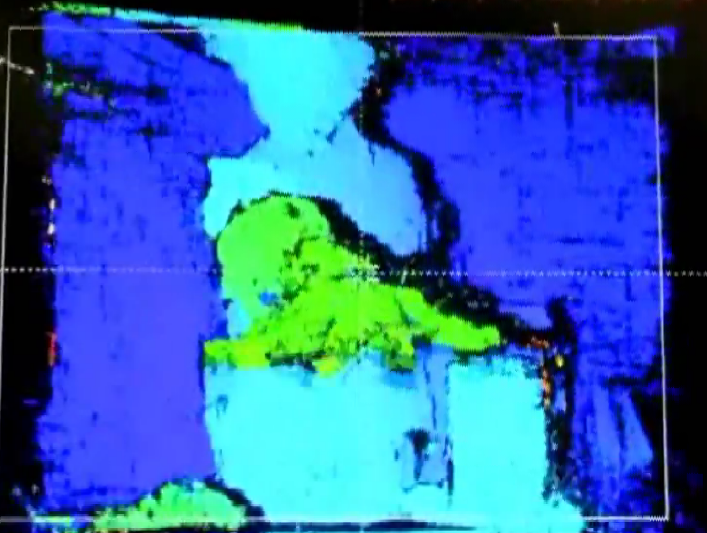
\includegraphics[scale=0.3]{EtronDepth.png}
  \caption{\label{etron} Depth map with two stereo camera}
\end{figure}

Stereo camera system is the cheaper system for retrieving a point cloud. It only requires some calibration and computation, but it is not a very expensive hardware compared to the other two systems.

The computed depth map is unfortunately very noisy. There is a lot of noise when we compute the depth map. Shadow effects can be seen on figure~\ref{etron}. Moreover it is very difficult to compute a distance for uniform area, since no feature information can be retrieved. We need to extrapolate the distance based  on the surrounding information, but this leads to low fidelity reconstruction of the scene.

\subsection{Conclusion}


\section{Design/Theory}
\subsection{KinectFusion}
For the reconstruction of the scene and the localization of the user, we use the KinectFusion algorithm. The KinectFusion algorithm achieves real-time dense surface mapping and reconstruction. The algorithm is fully described in \cite{KF1, KF2}. The GPU implementation of KinectFusion allows the real time reconstruction and localization. The algorithm is composed of four main stages:
\begin{enumerate}
\item \textbf{Depth Map conversion} The live depth map is converted into absolute 3D positions and normals in the camera coordinate space;
\item \textbf{Camera tracking} We keep a rigid 6 degrees of freedom transform of the camera. At time $i$, the camera pose is noted $T_i = [R_i|t_i]$ with $R_i$ being a 3x3 rotation matrix and $t_i$ being a 3D translation vector. We use the Iterative Closest Point algorithm for tracking the position and orientation of the camera.
\item \textbf{Volumetric integration}
\item \textbf{Raycasting} The volume is raycast to render the implicit surface.
\end{enumerate}

Each of this stage is performed in parallel on the GPU using CUDA.

\paragraph{Depth Map conversion} ~\\
The depth map is a 2D array of float. At time $i$, for each pixel $u(x,y)$ we have the corresponding depth $D_i(u)$. Given the calibration matrix $K$ of the Kinect infrared camera, we can compute the 3D position in the camera coordinate space. For each pixel $u$, a GPU thread compute the 3D position as follow:
$$v_i(u) = D_i(u)K^{-1}[u,1]$$
The results are saved in a single vertex map $V_i$.

We also compute the corresponding normal map, as it will be useful later for the ICP algorithm. Each normal $n_i(u)$ is computed by a GPU thread using the neighboring reprojected points:
$$n_i(u) = (v_i(x+1,y) - v_i(u))\times (v_i(x,y+1) - v_i(u))$$
The normal is then normalized and stored in a single normal map $N_i$.

Given the rigid body transform of the camera $T_i = [R_i|t_i]$, we can convert the vertices and the normals into global coordinates:
$$v_i^g(u) = T_iv_i(u)$$
$$n_i^g(u) = R_in_i(u)$$

\paragraph{Camera tracking} ~\\
Iterative Closest Point algorithm was introduced by \cite{ICP1}. It is a widely studied algorithm for 3D shapes alignement. \cite{ICP2} provides a detailed study of the ICP algorithm. In KinectFusion, ICP is also used for tracking the camera pose of the Kinect, that means its position and its orientation. For each new depth frame captured by the Kinect, the algorithm estimates the 6DOF transform that aligns the vertices and normals of the current frame with those of the previous frame. This gives a relative 6DOF transform. If we apply them together incrementally, we obtain the global camera pose $T_i$.

The first part of the ICP is to find correspondences between the current oriented points set at time $i$ with the previous one at time $i-1$. KinectFusion uses \textit{projective data association}. Given the previous global rigid body transform $T_{i-1}$

\paragraph{Volumetric representation and integration} ~\\

\paragraph{Raycasting} ~\\

\subsection{Oculus Rift Headtracking}

\subsection{Oculus Lens deformation}

\section{Implementation}
\subsection{kfusion}
\subsection{Lens deformation}
\subsection{Color rendering}
\subsection{Oculus Calibration}
\subsection{Magic Pen}

\section{Results}
\subsection{3D rendering}
\subsection{Magic pen}

\newpage
\section*{Conclusion}
\addcontentsline{toc}{section}{Conclusion}

\newpage
\addcontentsline{toc}{section}{References}
%\bibliographystyle{alpha}
%\bibliography{biblio}
\end{document}